\phantomsection
\section*{三、CEC 场景下的大模型推理}
\addcontentsline{toc}{section}{三、CEC 场景下的大模型推理}

\phantomsection
\subsection*{3.1 CEC LLM 推理的系统形态}
\addcontentsline{toc}{subsection}{3.1 CEC LLM 推理的系统形态}

CEC 场景下的大模型推理运行在由多个地理分布、能力异构的边缘节点组成的协作系统中 \cite{duan2022distributed}。协作节点可以是具备推理能力的终端设备、边缘服务器和 AI 板卡，也可以是部署在基站、网关或园区中的推理实例；请求可从终端、基站或边缘网关等任一入口进入。模型权重、adapter（参数高效微调模块）、KV Cache、prefix cache、session state 和中间状态可以集中在单个节点，也可以分布在多个协作节点上。一次推理既可以在本地实例内完成，也可以通过节点间的计算与状态传输协同完成；外部云服务仅在具体业务允许时作为可选服务或回退路径。

与云侧集中式 LLM serving 相比，CEC 的主要变化是执行范围从单个实例或集中式集群扩展到分布式边缘资源池。云侧 serving 通常具有相对集中的资源和稳定互联，优化重点是单实例或集群内部的吞吐、显存和调度效率。CEC 还需要把节点位置、无线与边缘网络、异构硬件、移动接入、状态分布和隐私边界纳入推理路径。推理系统需要同时确定执行实例、跨节点模型部署、状态保留位置、节点间传输方式和服务路径调整条件。图~\ref{fig:cec-llm-serving-architecture} 展示了模型分割部署、计算任务调度和 KV/runtime state 调度在协作边缘节点之间的关系。

\begin{figure}[!htbp]
    \centering
    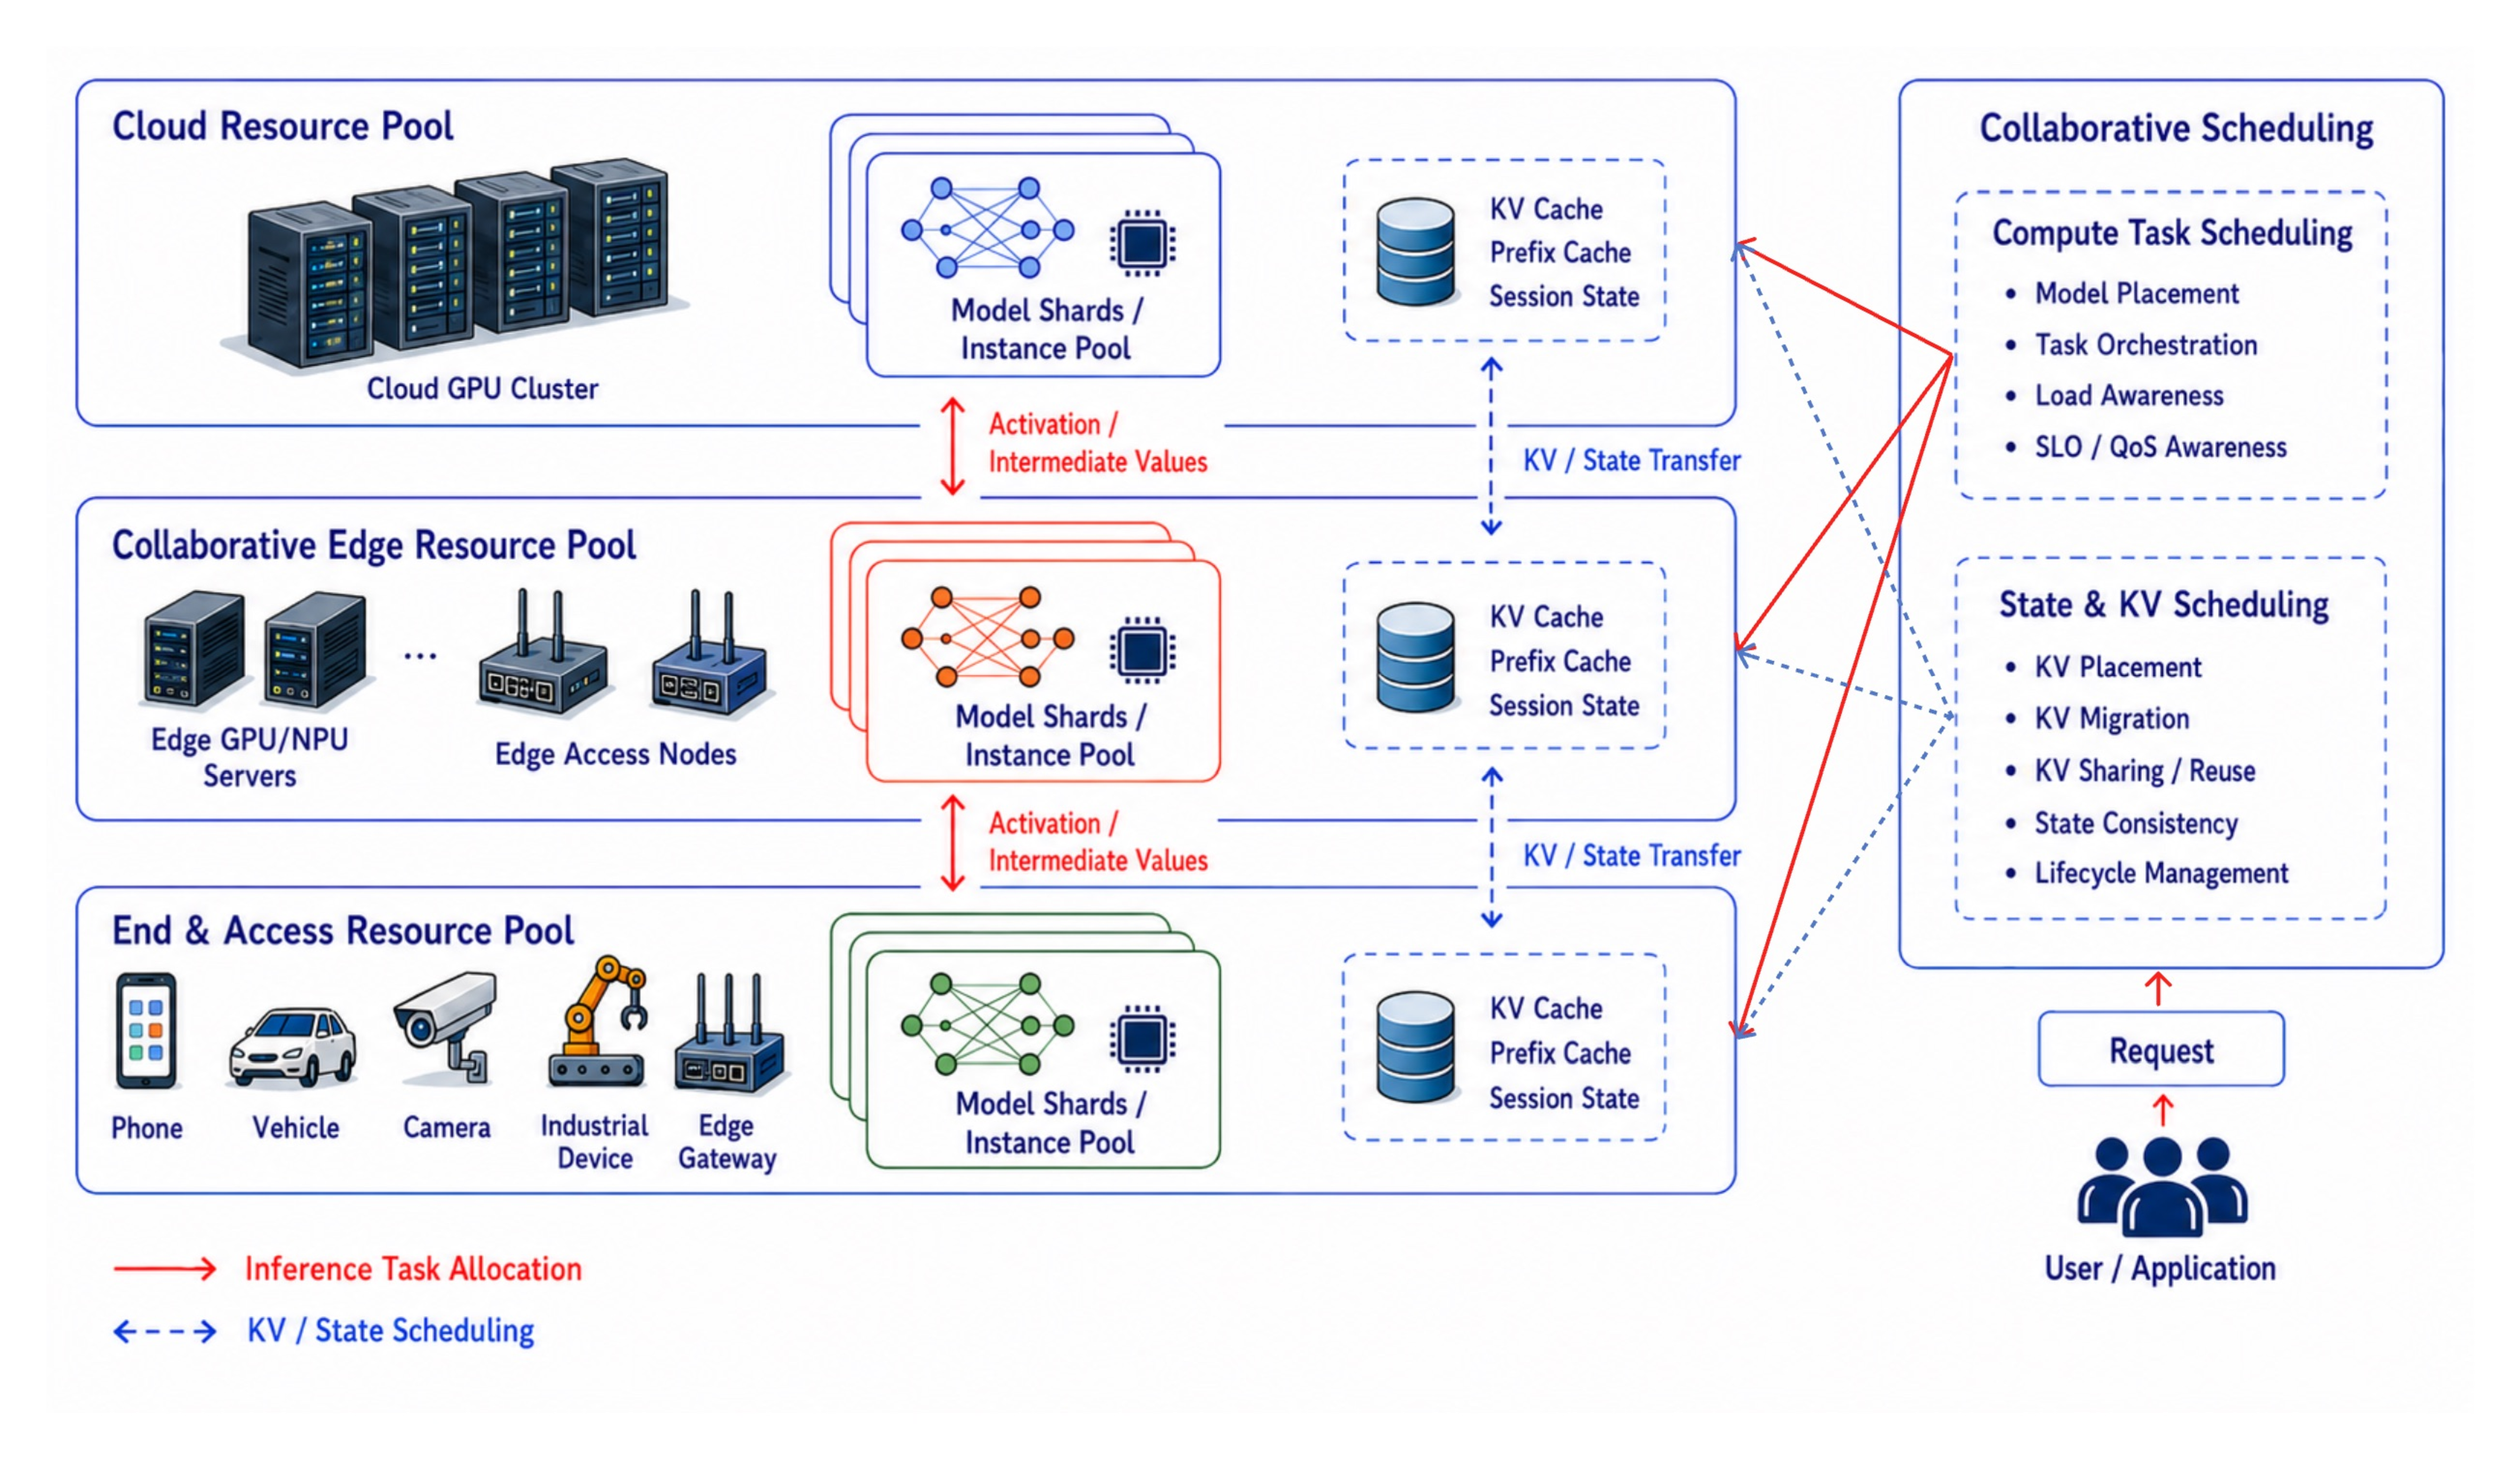
\includegraphics[width=\textwidth]{figures/ch3_cec_llm_serving_architecture.pdf}
    \caption{\textbf{CEC 环境下的 LLM 推理 Serving 系统形态。}Serving Policy 根据协作节点的资源、链路与运行状态，协调模型分割与部署、Prefill/Decode 等计算任务调度，以及 KV Cache、Prefix Cache 和 Session State 的复用、迁移与远程访问。}
    \label{fig:cec-llm-serving-architecture}
\end{figure}

CEC LLM inference 主要包含三类相互关联的决策。模型部署决定模型的哪些部分由哪些协作节点执行；实例内调度决定请求如何组成 batch，以及 prefill 和 decode 如何安排；服务路径选择决定请求、会话和运行时状态在协作节点之间如何路由、迁移或复用。后续章节分别围绕这三类问题展开。

\phantomsection
\subsection*{3.2 CEC 相较云侧集中式 LLM Serving 新增的约束}
\addcontentsline{toc}{subsection}{3.2 CEC 相较云侧集中式 LLM Serving 新增的约束}

\textbf{资源受限与硬件异构：}模型规模、KV Cache、batching、并行执行和多实例调度在云侧同样存在，CEC 则进一步面临单节点资源受限和设备能力差异。协作资源池中的终端设备、边缘服务器和 AI 板卡在算力、显存、内存、功耗及散热预算上差异明显，同一个模型未必能完整放入目标设备；即便容量足够，也可能受到低比特算子、算子覆盖范围、推理后端和数据布局转换的限制。因此，部署方案必须同时考虑设备容量、实际执行能力和节点间通信。

\textbf{网络波动与状态移动成本：}终端接入链路和边缘节点间链路的带宽、RTT、抖动与拥塞状态会直接影响模型切分、task offloading、prefill/decode 分离和 KV 迁移是否值得执行。对于普通 DNN 推理，跨节点传输的主要对象通常是输入或中间 activation；而在 LLM inference 中，KV Cache、prefix cache、session state 和多轮上下文也会成为需要迁移或远程访问的状态资源。网络成本因此不再只是请求入口到服务实例的传输延迟，而是贯穿推理全过程的状态移动成本。

\textbf{请求负载突发且SLO要求异构：}单个请求入口附近的边缘节点通常资源受限，请求到达具有突发性，并且不同请求的SLO要求各不相同。等待较大的 batch 会增加 TTFT，完全放弃 batching 又会降低 GPU/NPU 利用率。prefill 与 decode 的资源需求不同，长短请求和不同 SLA 请求混合到达时，固定 batch size 与 FIFO 队列很难同时保证吞吐和尾时延。因此，边缘运行时需要根据当前队列、请求时限、KV 占用和阶段负载动态调整组批与执行顺序，以满足不同请求的SLO要求。

\textbf{用户移动与服务连续性：}对于单轮短请求，移动可能只改变入口节点；对于多轮对话、长上下文和 agent workflow，移动会改变服务实例与状态位置之间的关系。KV Cache、prefix cache、session state 或 agent memory 可能仍然停留在原服务节点，新请求却已经从新的入口进入系统。系统需要在迁移状态、远程访问原有状态、重新 prefill 或缩短可用上下文之间做选择。因此，评价指标还需要覆盖会话连续性、状态复用和移动场景下的 QoS 稳定性。

\textbf{隐私边界与数据本地性：}部分 prompt、传感器数据、业务上下文或用户状态可能不能离开本地边缘域，也可能只允许在指定节点集合内流动。隐私约束会限制模型选择、offloading 范围、KV 迁移路径和 fallback 策略，使系统不能仅按最小时延或最低成本选择节点。换言之，CEC 中的推理优化必须同时处理资源可行性、链路代价、状态位置、隐私边界和业务 QoS。

\phantomsection
\subsection*{3.3 现有 LLM Inference 优化在 CEC 中的关注重点}
\addcontentsline{toc}{subsection}{3.3 各类 LLM Inference 优化在 CEC 中的关注重点}

\textbf{Model-Level：关注模型表示与结构能否适配目标设备。}量化、剪枝和小模型替代会改变模型的容量与计算需求，GQA、MoE 等结构还会影响 KV 大小、条件计算和通信模式。模型结构是否便于按 layer、tensor 或 expert 拆分，会影响跨节点部署的可行性；具体分割位置、并行度和执行顺序则由分布式 Runtime 决定。

\textbf{Kernel-Level：关注异构硬件的算子支持与执行效率。}CEC 系统可能同时包含不同规格的 NPU、GPU、CPU 及 AI 板卡。各后端支持的数据精度、算子、attention kernel、KV 布局和通信原语并不一致。一个模型在数据中心 GPU 上能够高效执行，并不意味着它在边缘设备上具有相同性能；不受支持的算子、数据布局转换和 CPU 回退都可能抵消协同执行的收益。

\textbf{Runtime-Level：把网络和状态纳入在线执行控制。}云侧 runtime 主要管理单个 serving engine 或集中式集群内的 KV、batch 和执行流水线；CEC runtime 还要读取链路状态、节点负载、KV 位置和用户入口变化。KV 管理由单实例显存分配扩展为跨节点状态管理，batching 需要适应SLO要求异构且动态的请求池，分布式执行则要同时安排节点计算和跨节点数据传输。

\textbf{Serving Policy \& Routing-Level：联合选择执行节点和状态处理方式。}一个请求是在入口节点执行，还是交给其他协作节点，需要同时考虑模型可用性、链路状态、节点负载、KV/cache 位置、用户入口变化、隐私限制和 SLA 风险。除选择执行节点外，服务策略还要决定状态是本地复用、跨节点同步、远程访问还是重新计算。

在 CEC 中，模型部署、运行时调度和服务路径选择共享同一组设备、链路和状态条件。模型切分决定执行拓扑和通信量，batching 改变实例容量与排队时间，KV 状态位置又会影响请求卸载代价。基于这种关系，后续章节按模型切分、业务感知 batching 和请求卸载三类具体问题组织相关工作与方案。

\phantomsection
\subsection*{3.4 本文采用的 CEC LLM Inference 综述框架}
\addcontentsline{toc}{subsection}{3.4 本文采用的 CEC LLM Inference 综述框架}

基于上述分析，本文将 CEC 场景下的 LLM inference 优化归纳为三条主线。第一条是资源自适应模型部署，对应模型计算如何分配到协作节点。第 4 章的相关工作综述覆盖 layer-wise、tensor/operator-level、expert/component-level、inference phase 和 semantic/token-level partitioning；面向验证环境的方案则用统一代价模型比较 TP、PP 和 PP+TP，并采用动态规划求解非均匀 PP 的连续 layer 边界。

第二条是业务感知 batching，对应请求进入推理实例后的组批与执行顺序。第 5 章先分析 dynamic batching、continuous batching、chunked prefill 和 prefill/decode 分池等机制，再将在线控制建模为 CMDP，采用带拉格朗日风险约束和安全投影的 Safe-RL 调节 batch 容量、请求排序和运行时机制。

第三条是 LLM inference task offloading，对应跨节点服务路径选择，关注完整请求、会话、复杂 workflow 以及 context、KV Cache、prefix cache 和 session state 如何在协作节点之间路由、同步、复用或重新计算。第 6 章在相关工作综述后，进一步给出联合选择执行节点和 KV 获取方式的长期会话感知方案。

如图~\ref{fig:cec-taxonomy} 所示，这三条主线分别从空间部署、时间调度和服务路径三个角度刻画 CEC LLM inference 的关键优化问题。它们并非彼此独立：模型部署决定可用的执行拓扑，batching 决定实例内部的时间组织，task offloading 决定请求和状态如何在协作网络中移动。第 7 章将进一步讨论三类算法之间的协同优化关系。

\begin{figure}[!htbp]
    \centering
    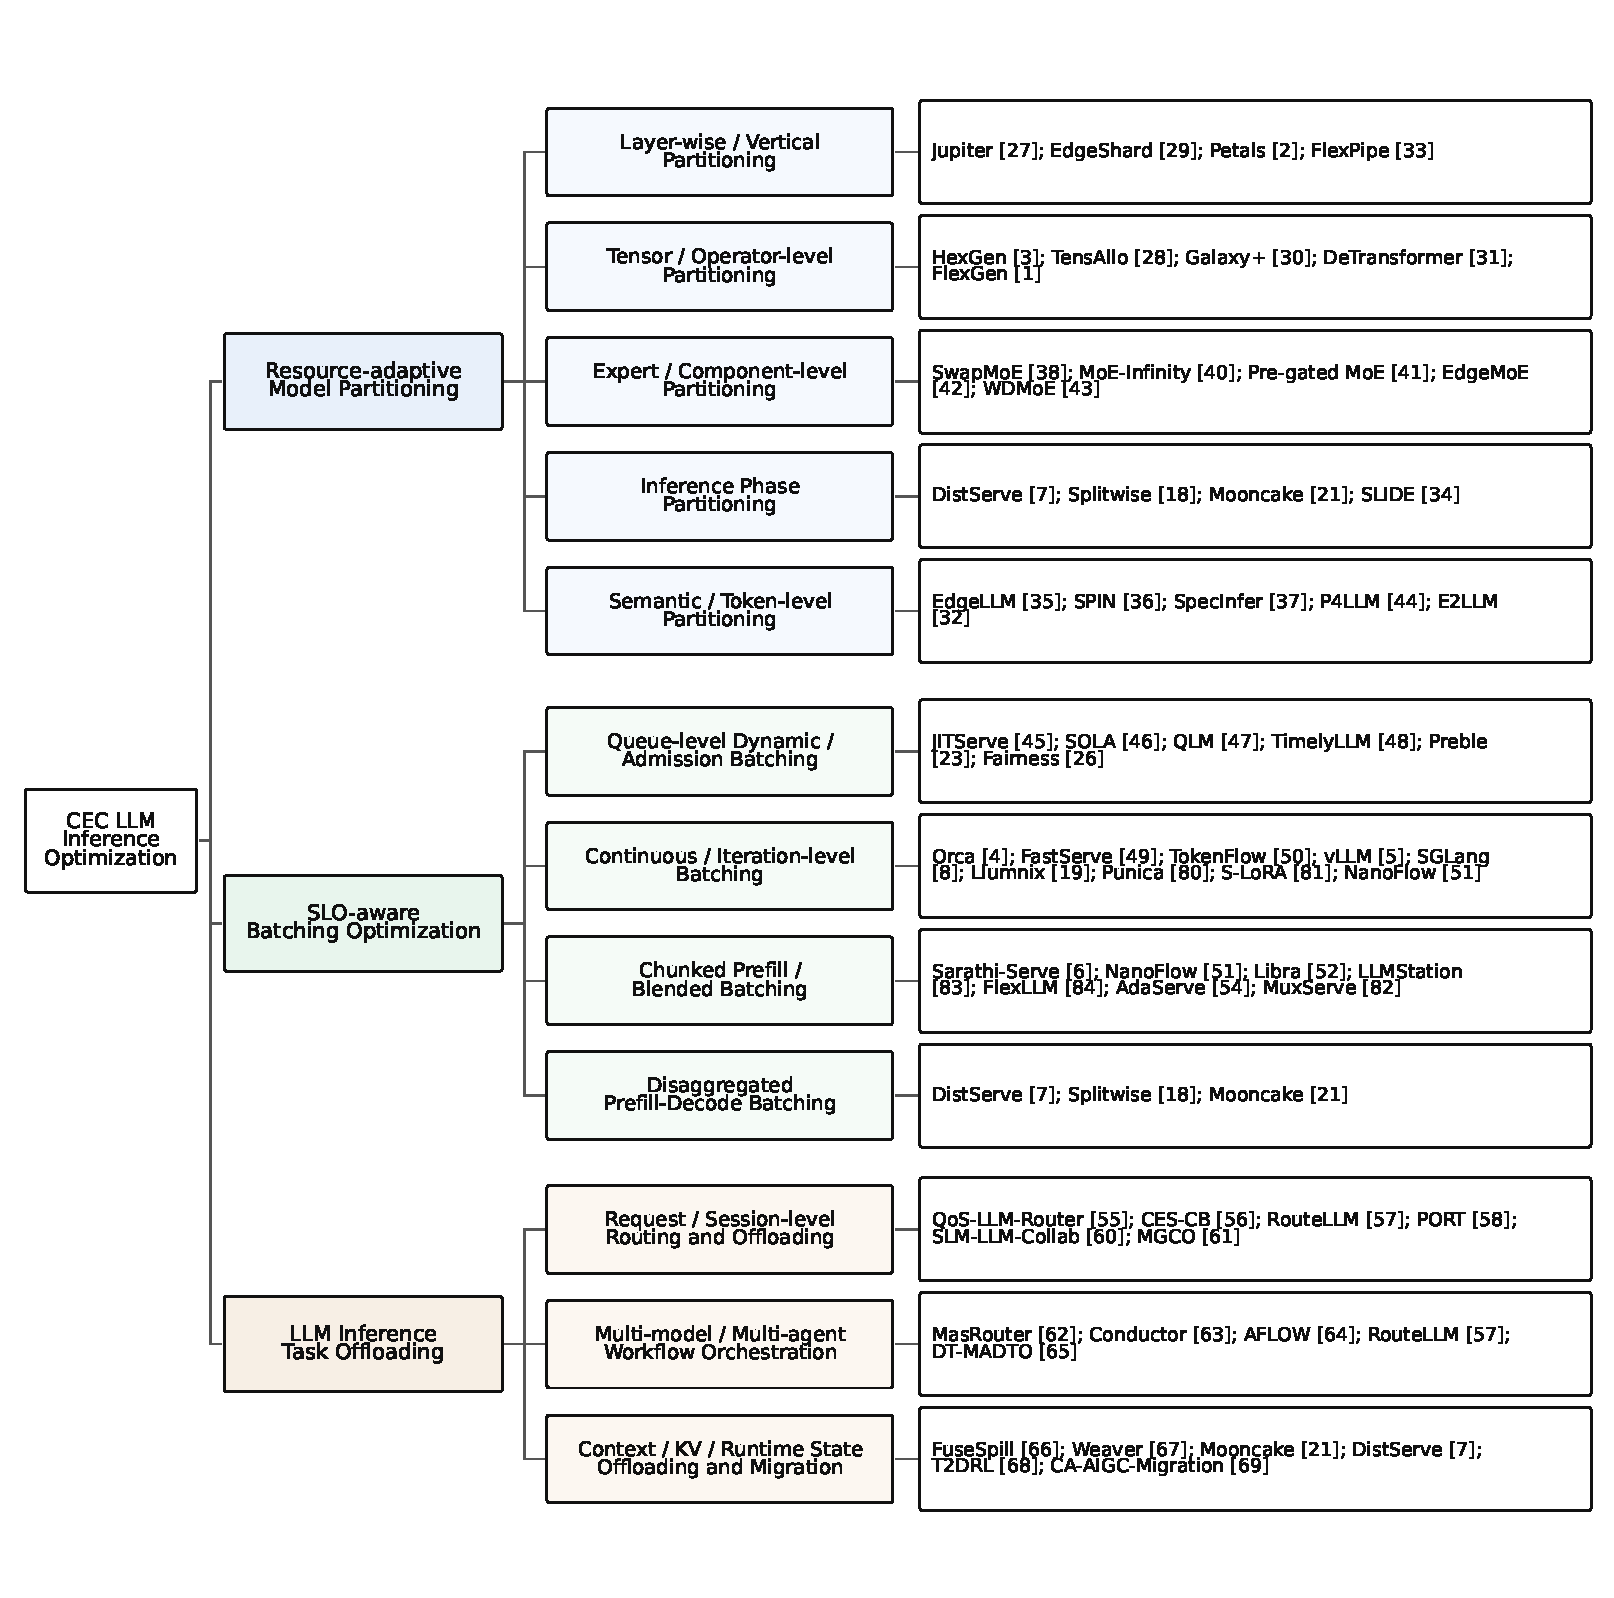
\includegraphics[width=\textwidth]{figures/cec_llm_optimization_overview_taxonomy.pdf}
    \caption{\textbf{CEC LLM inference 优化主线、子分类与代表工作总览}}
    \label{fig:cec-taxonomy}
\end{figure}

\phantomsection
\subsection*{3.5 小结}
\addcontentsline{toc}{subsection}{3.5 小结}

本章从系统形态出发，说明 CEC LLM inference 由多个异构边缘节点协作提供服务。相较数据中心环境，CEC 需要进一步处理资源异构、网络波动、局部请求池规模有限、用户移动、状态连续性和隐私边界等约束，使模型部署、实例内调度和跨节点服务路径使用一致的资源与状态信息。

按照“优化对象--执行范围”分类，CEC 中的 Model-Level 更关注模型表示和结构能否适配目标设备，Kernel-Level 更关注异构硬件的算子支持与执行效率，Runtime-Level 需要同时管理模型切分执行、网络、状态、batch 和执行流水线，Serving Policy \& Routing-Level 则联合选择执行节点与状态处理方式。

基于这些变化，本报告后续围绕三类 CEC LLM inference 优化主线展开：CEC 下的资源自适应模型部署方法、CEC 中的业务感知 batching 参数优化算法，以及 CEC 中的 LLM inference task offloading。
